\section{Auswertung}
\label{sec:Auswertung}

Der Abstand der Kondensatorplatten beträgt
\begin{align}
  d = (7.6250 \pm 0.0051) \si{\milli\m} \; .
\end{align}
Die gemessenen Geschwindigkeiten befinden sich in Tabelle~\ref{tab:v}. Es wurde die Zeit gemessen, die ein Tröpfchen benötigt um eine gewisse Anzahl an Kästchen zu durchlaufen. Über
\begin{align}
  v = \frac{s}{t}
\end{align}
kann damit die Geschwindigkeit ermittelt werden. Wobei der Weg
\begin{align}
  s=\mathrm{Kästchenanzahl} \cdot \SI{0.5}{\milli\m}
\end{align}
beträgt.

Es war nicht für jedes Tröpfchen möglich $v_0$ zu bestimmen, daher konnten nur sehr wenige Tröpfchen auf Grund der Beziehung
\begin{align}
  \label{equ:test}
  2 v_0 = v_{\mathrm{ab}} - v_{\mathrm{auf}}
\end{align}
aussortiert werden. Auch mit der Annahme einer Messungenauigkeit von $25\%$ fallen damit alle Tröpfchen weg, für die überhaupt $v_0$ gemessen wurde.
Als nächstes werden alle Geschwindigkeiten, die zu einem bestimmten Tröpfchen gehören, mit Hilfe von Gleichung~\eqref{equ:mean} und \eqref{equ:stdofmean} gemittelt und die geschätzte Standardabweichung des Mittelwerts berechnet.


 \begin{table}
   \centering
   \caption{Geschwindigkeiten der Öltröpfchen mit zugehöriger angelegter Ladung. Eine nicht vorliegende Messung ist durch den Wert 0 gekennzeichnet.}
 \label{tab:v}
   \sisetup{table-format=1.0}
   \begin{tabular}{
       S[table-format=3]
       S[table-format=1.2]
       S[table-format=2.2]
       S[table-format=2.2]
       }
       \toprule
        $\text{Spannung in V}$ & $\text{$v_0$ in $10^{-5} \si{\m\per\second}$}$ & $\text{$v_{\mathrm{ab}}$ in $10^{-5} \si{\m\per\second}$}$
        & $\text{$v_{\mathrm{auf}}$ in $10^{-5} \si{\m\per\second}$}$\\
       \midrule
       \primitiveinput{../tex-data/v.tex}
       \bottomrule
   \end{tabular}
 \end{table}

Mit Gleichung~\eqref{equ:ladung} kann nun aus den gemittelten Werten die unkorrigierte Ladung $q_{\mathrm{unkorr}}$ berechnet werden.
Die dafür benötigte unkorrigierte Viskosität wird über den Thermistor-Widerstand bestimmt. Aus der Tabelle in Abbildung~\ref{fig:T} kann daraus die Temperatur abgelesen werden und aus Abbildung~\ref{fig:eta} die daraus resultierende Viskosität:
\begin{align}
  \Omega_{\mathrm{anfang}} &= 1.86 \si{\mega\ohm} &\to 28 \si{\celsius} &\to \eta_{\mathrm{L}} = \SI{1.862e-5}{\newton\second\per\square\m} \\
  \Omega_{\mathrm{ende}} &= 1.82 \si{\mega\ohm} &\to 29 \si{\celsius} &\to \eta_{\mathrm{L}} = \SI{1.8665e-5}{\newton\second\per\square\m} \; .
\end{align}

\begin{figure}[H]
  \centering
  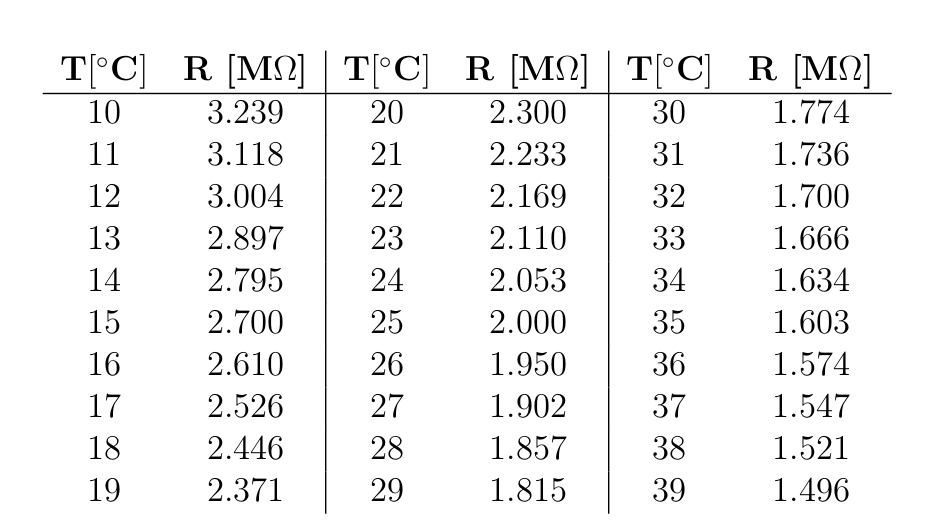
\includegraphics[width=0.4\textheight]{../figures/tab.png}
  \caption{Thermistor-Widerstandstabelle. [Skript V503]}
\label{fig:T}
\end{figure}

\begin{figure}[H]
  \centering
  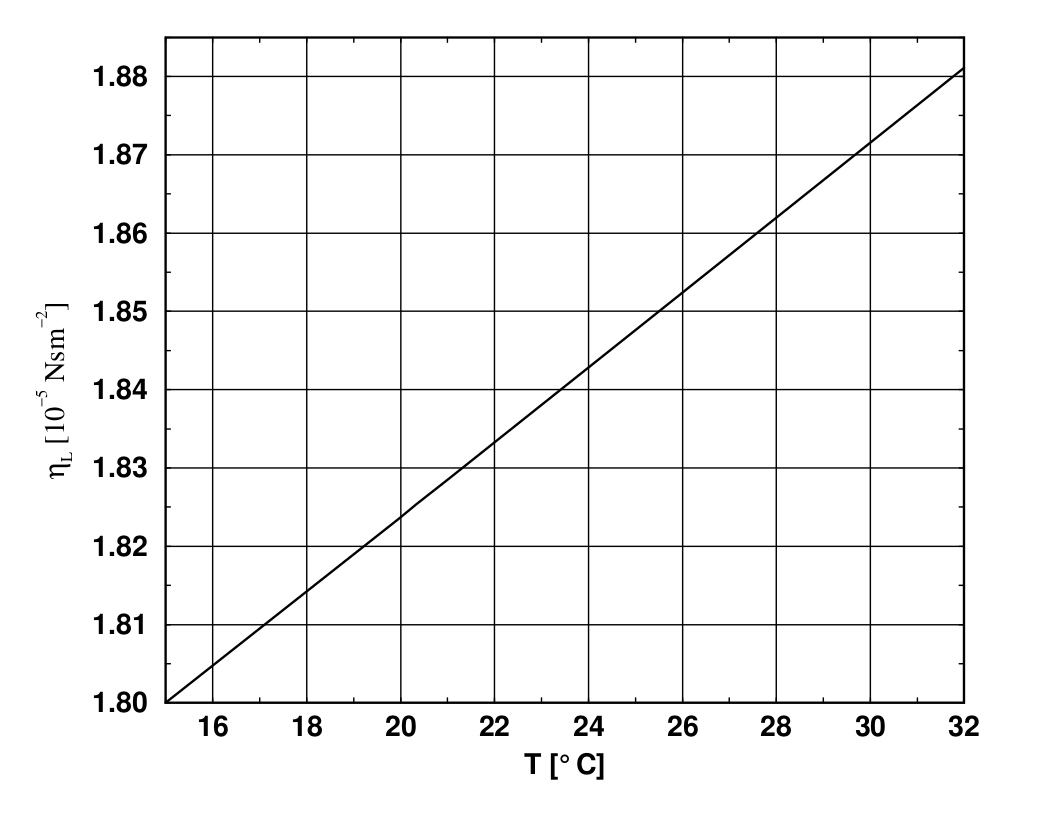
\includegraphics[width=0.4\textheight]{../figures/eta.png}
  \caption{Die Viskosität $\eta$ von Luft als Funktion der Temperatur. [Skript V503]}
\label{fig:eta}
\end{figure}

Die Viskosität kann nun nach Cunningham mit Gleichung~\eqref{equ:cunning} korrigiert werden, wodurch sich die korrigierte Ladung für jedes Tröpfchen ergibt. Der Cunningham-Korrekturterm beträgt $B = 6.17~\cdot~10^{-3} \si{\torr\cm}$ [Skript V503]. Die korrigierte Ladung $q_{\mathrm{korr}}$ ist in Abbildung~\ref{fig:ladung} gegen die Tröpfchennummer aufgetragen, die Werte sind in Tabelle~\ref{tab:q} zu finden.

\begin{figure}[H]
  \centering
  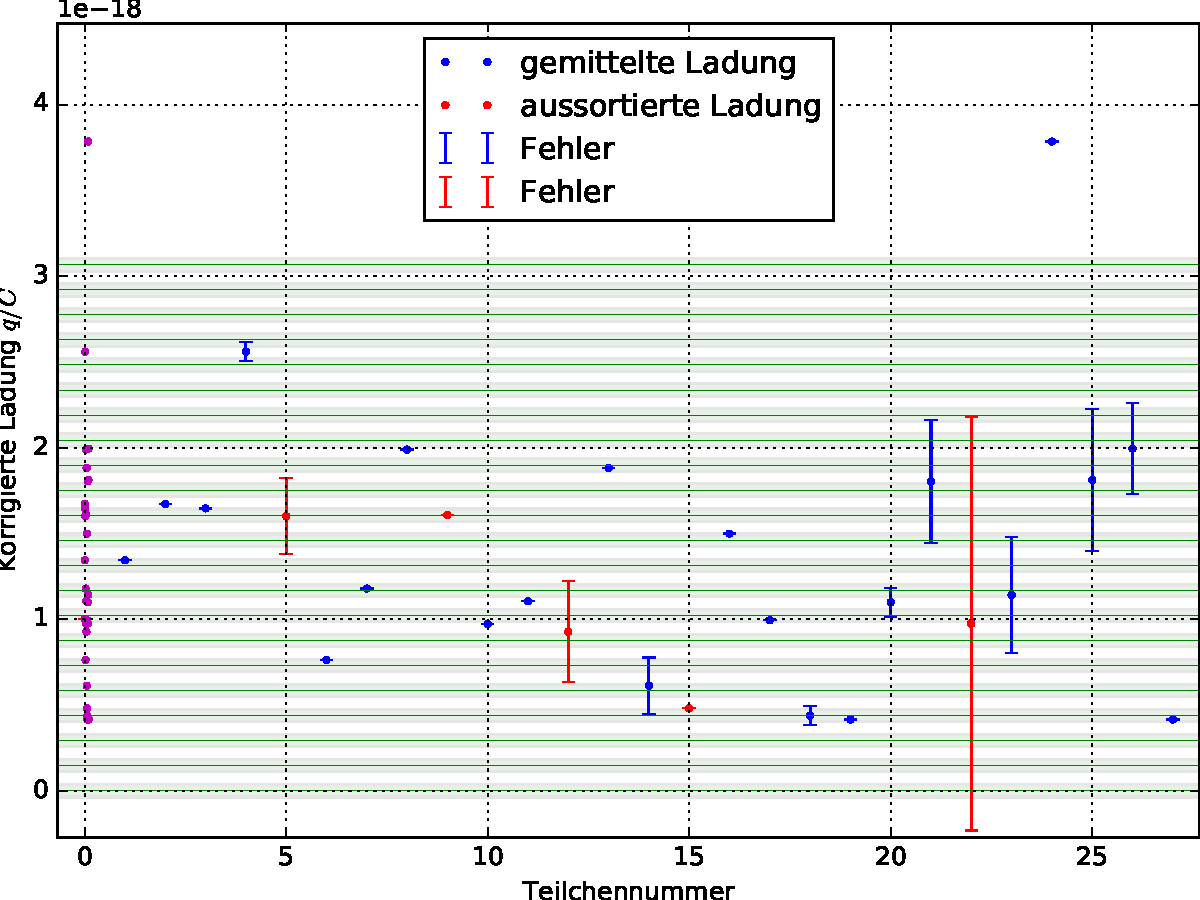
\includegraphics[width=0.5\textheight]{../plots/ladung3.pdf}
  \caption{Plot der korrigierten Ladungen gegen ihre Teilchennummer mit grünen Niveaulinien der ermittelten Elementarladung. Zu Vergleichszwecken sind die gemittelten Ladungen zusätzlich in Magenta auf eine Linie geplottet worden.}
\label{fig:ladung}
\end{figure}

\begin{table}[H]
  \centering
  \caption{Gemittelte Ladungen $q$ und korrigierte Ladungen $q_{\mathrm{korr}}$.}
\label{tab:q}
  \sisetup{table-format=1.0}
  \begin{tabular}{
      S[table-format=8.5]
      @{${}\pm{}$}
      S[table-format=1.6]
      S[table-format=8.5]
      @{${}\pm{}$}
      S[table-format=1.6]
      }
      \toprule
      \multicolumn{2}{c}{$\text{$q / 10^{-19}$ C}$} & \multicolumn{2}{c}{$\text{$q_{\mathrm{korr}} / 10^{-19}$ C}$}\\
      \midrule
      \primitiveinput{../tex-data/q.tex}
      \bottomrule
  \end{tabular}
\end{table}

Mit Hilfe einer leichten Abwandlung des Euklidischen Algorithmus (siehe Abbildung~\ref{fig:eukl}) lässt sich nun aus den korrigierten Ladungen ein größter gemeinsamer Teiler bestimmen, der die Elementarladung $e_0$ darstellen soll.

\begin{figure}
  \centering
  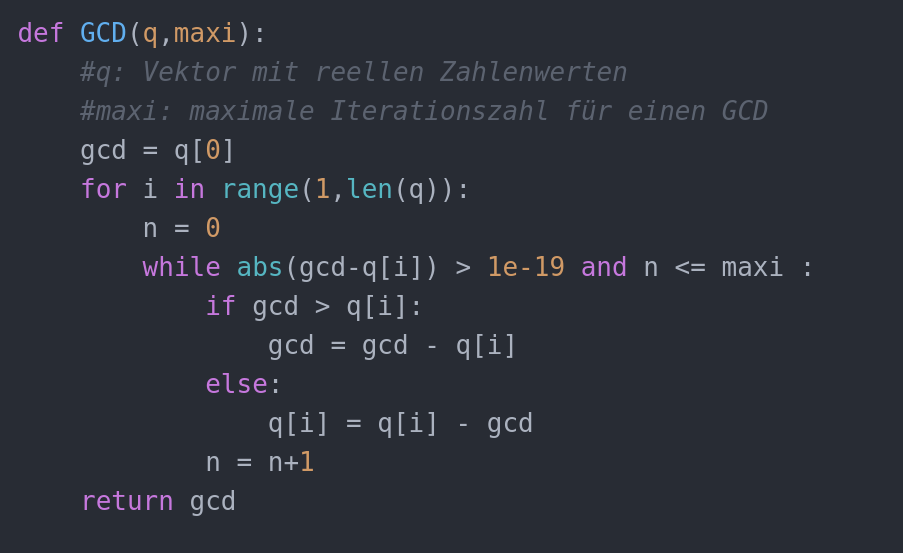
\includegraphics[width=0.5\textheight]{../figures/GCD.png}
  \caption{Sourcecode des benutzten geänderten Euklidischen Algorithmus in \emph{python}.}
\label{fig:eukl}
\end{figure}

Aus den Daten ergibt sich mit diesem Code für die Elementarladung
\begin{align}
  e_0 = (1.46 \pm 0.25)\cdot 10^{-19} \si{\coulomb} \; .
\end{align}
Sie weicht von der tatsächlichen Elementarladung $e_{0,\mathrm{theorie}}~=~1.602~\cdot~10^{-19}~\si{\coulomb}$  um ca. $8.8\%$ ab. Die Niveaulinien, die sich aus der berechneten Elementarladung ergeben, sind in Abbildung~\ref{fig:ladung} mit einer Abweichung von $25\%$ in grün eingezeichnet.
Die Avogadrokonstante berechnet sich mit Hilfe der Faraday-Konstante ($F~=~\SI{96485.33289}{\coulomb\per\mol}$) und der bestimmten Elementarladung zu
\begin{align}
  N_A = \frac{F}{e_0} = \SI{6.6086e+23}{\per\mol} \; .
\end{align}
Die Abweichung zum Theoriewert $N_{\mathrm{A,theorie}}~=~\SI{6.022140857e+23}{\per\mol}$ beträgt ca. $9.7\%$.

%the end
